\documentclass{article}
\usepackage[utf8]{inputenc}
\usepackage{graphicx}

\usepackage[
	citestyle=ieee, 
    bibstyle=ieee,
    style=numeric-comp,
]{biblatex}
    
\addbibresource{ref.bib}


\title{The necessity of Microservices in a DevOps environment}
\author{
{Julius Celik}\\
\textit{
    jcelik@kth.se
} \and {Patric Ridell}\\
\textit{
    pridell@kth.se
}}
\date{\today{}}

\setlength{\parindent}{0em}
\setlength{\parskip}{1em}

\begin{document}

\maketitle

% 10 Tech Challenges That Are Solved by Microservices
% https://medium.com/containerum/10-tech-challenges-that-are-solved-by-microservices-d91adeecb2e7

\section{Introduction}
Microservices is a software development method, where systems are divided into smaller parts, called microservices, that can be individually deployed. In turn, this enables low coupling, high cohesion, and strong composibility. The microservices are focused on performing single tasks really good, and implementing functionality by composing multiple microservices. It also enables multiple developers to work on a common codebase while minimizing obstruction, which becomes more notable in larger systems, with more developers.

The opposite of microservice are often called monoliths. A monolith is a whole system implemented as a single application. This means that the system is always handled as a single entity, which in practice means that the whole system has to be running to perform integration tests on parts of the system, and the whole application is duplicated when the system is scaled in a distributed manner.

Microservice developed as a natural response to agile organizational structures. Agile development has become the industry norm for software development \cite{Jeremiah}. This means that companies organize their software developers in smaller teams of usually four to eight developers, where the teams have full life cycle ownership of the software they write. Conway's law states that:
\begin{quote}
    Any organization that designs a system (defined broadly) will produce a design whose structure is a copy of the organization's communication structure. \cite{Conway}
\end{quote}

As organizations divide software developers into self managed teams, Conway's law implies that it is a natural progression to divide the systems into decoupled services that can be independently deployed.

% The problem with monoliths
% https://smartbear.com/solutions/microservices/


\section{Benefits of microservices within DevOps}
% The difficulties of using a CI on a large monolith. Every change triggers a rebuild/retest of everything
In a monolith application, there is an ever increasing difficulty for \textit{Continuous Integration} (CI). With every small modification of the codebase, one might have to build and deploy an entire new version of the application \cite{Jeremiah}. This section will explore how microservices tackle this problem and in what ways they enable CI, a foundation of DevOps. We will see that in most cases, DevOps and microservices go hand-in-hand and augment each others functionality.

\subsection{Microservices enable individual deployments}
% All or nothing deployments. Individual deployments
At the core of microservices is modularity; doing one specific task really well. A consequence of the modular nature of microservices is the possibility of individual deployments. For some developers like \citeauthor{Newman2015} the ability to individually deploy microservices is one of the fundamental definitions of microservices \cite{Newman2015}.

When a system becomes so large that multiple teams of developers work on it, changes to the system are done very frequently. If the teams use agile methods like CI the work done by every developer should be merged into a shared repository multiple times a day. With many people working on the same application that becomes hundreds or thousands of merges every day. At a certain point it becomes impossible for every change to trigger a new run of the CI-pipeline, as the CI would be overloaded where multiple new updates comes as the CI executes a single run. This leads to multiple problems when deploying releases.

\subsubsection{Large-impact and high-risk deployments}
The difficulty of releasing a monolith creates multiple problems. One problem is that the deployments become larger and take longer time. It is also more difficult to deploy a large monolith compared to a microservice. \citeauthor{Newman2015} highlights the potential for such a deployment to be \textit{large-impact} and \textit{high-risk}. \citeauthor{Newman2015} claims that this leads to deployments happening infrequently due to understandable fear. This leads to larger changes between releases, which develops a higher risk for something wrong to be released. \cite[p.~6]{Newman2015}

Infrequent deployments lead to larger software-deltas and longer feedback loops. When something wrong happens it is difficult to understand why it is wrong because it might have been a long time since the change was implemented, and there might be many changes since the last release.

\subsubsection{Fault management and automation}
Another problem that is related to releasing monoliths is the ability to use rollbacks, and the use of \textit{Continuous Deployment} (CD). For the reasons mentioned above it is difficult and often impossible to use CD, and when a faulty system is released, it is often difficult to rollback the system to a previous stable version.

With microservices it is easy to release every minor update of the service, and to release often. It is therefore very easy to automate releases with CD's as well as managing releases with canary releases, where the update is only deployed on a small percentage of the servers, or exposed to a small percentage of users, and predefined metrics are verified to be sufficient before deploying the change to all of the servers. Canary releases require a measurable goal to be defined, like all requests to a service should be responded to within 500ms. With a microservice one or a few metrics can be defined and measured for every microservice. For a monolith that would require a very large amount of metrics to be measured, which would be difficult to both maintain and measure.


\subsection{Quicker feedback loops with fine grained modular testing}
% Quicker testing of parts of system. Feedback loop.
Decreasing the time between the releases of new features is a highly valuable trait within the DevOps development cycle. Microservices enable this through quicker feedback loops that allow testing of smaller and more specific parts of the system.

When testing a monolith parts of the application can not be mocked, which means that even to test a part of the system, the whole system has to be initiated. This leads to large overhead for smaller integration tests, and also difficulties in testing parts of the system.

One benefit of using microservices is that tests can be performed quicker, which enables a quicker feedback loop. The other benefit is that parts of the system only can be unit tested, or not tested at all. To test parts of a system, with integration tests, is crucial to maintain high quality software, and to align with DevOps methods.

\subsection{Scalability}
% Automatic scalability
The architecture used within an application can either work as a bottleneck on the growth of the application or be a tool that enables expansion. Although it is certainly possible to maintain a large monolith system, there a definitely easier and more effective ways. To scale a monolith service, every part of it has to be scaled simultaneously \cite{Newman2015}. Microservices allows a developer to prepare for future expansion by making the architecture more scalable. A developer can scale a specific service where it is needed, while leaving others unchanged \cite{Newman2015}.

\subsection{Decoupling team dependencies}
When developing a monolith system there is always a risk that coupling creeps into the codebase by multiple modules using the same database tables, business logic being implemented in shared libraries, or implementations not being abstracted enough. When a team wants to change a part of the code that has multiple dependants in code maintained by other teams, it requires that the different teams coordinate. These coordinated efforts can take months to implement, and as it often requires multiple people to discuss the changes over multiple meetings. This is a task that can not be solved with automation which would be the desirable DevOps solution.

Of course coupling can appear in microservice systems both by multiple services using the same database tables or business logic being implemented in shared libraries. It is however a lot easier to identify and avoid. The difference between a shared library used by multiple microservices compared to used in multiple parts of a single application is a much clear distinction. It is also very easy to avoid multiple microservices using the same databases as it is clearer to understand when only one microservice uses a database, versus only a distinguished part of an application uses a database. Coupling is also avoidable for monoliths, however it is not as easy, and monolith systems are often very coupled.

With microservices and the concept of individual deployments these team dependency problems are largely avoided. This is why individual deployments are so fundamental to microservices. If a team wants to change the implementation of their microservice it does of course not affect any other teams, as one can be certain that other teams only depend on your microservices interface. If a team wants to update the interface of a microservice the team can deploy both an old version and a new version of the microservice, or just two interfaces to the same service. Other teams get to migrate to the new version of the updated service gradually. When all dependants have migrated to the new version of the microservice the old version can be removed. This is shown in figure \ref{fig:microservice-versioning}.

This migration method is only possible to accomplish with microservices, and completely eliminates the previous problems with team dependencies. This enables teams to move quicker and be less dependant of each other. It is a requirement for DevOps practices like CI and CD to be used.

\begin{figure}
    \centering
    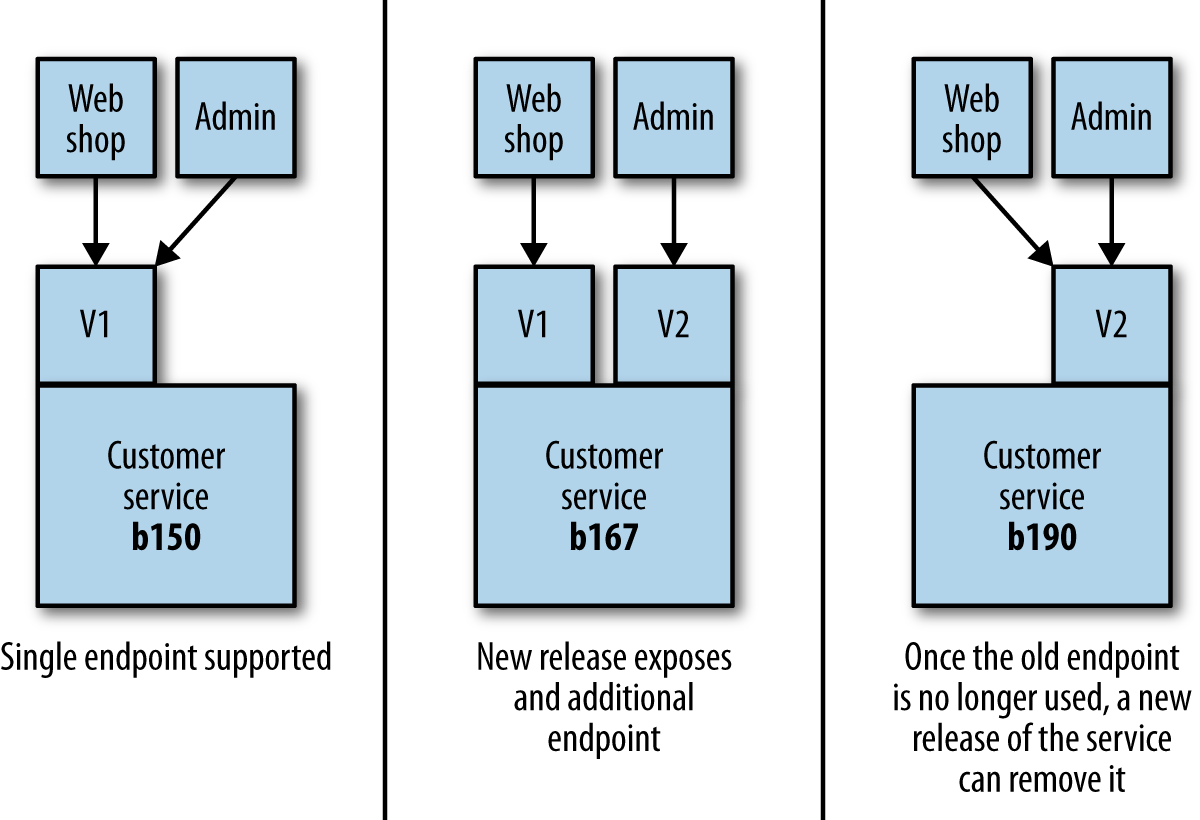
\includegraphics[width=\textwidth]{microservice-versioning.png}
    \caption{``\textit{Coexisting different endpoint versions allows consumers to migrate gradually}'', borrowed from \cite{Newman2015}}
    \label{fig:microservice-versioning}
\end{figure}


\section{Potential pitfalls}

% Distribution is difficult
% Automatic service discoverability
% Changing the architecture is painful
% Bad patterns like high coupling can magnify old problems with orders of magnitude

\section{Conclusion}
This short essay only scratches the surface on why microservice is a necessity for using DevOps practices. We introduced some concrete examples of why this is the case, as well as explained how to use microservices in practice for DevOps.

% Why microservices are essential to DevOps
Although there are some potential risks that a developer should be aware of when using microservices, they are far outweighed by the possibilities microservices bring. A major factor in staying competitive in any IT-related field is being \textit{first}. The early bird gets the worm. Being able to reduce time in-between iterations and quickly adapt to a changing business environment is essential for the longevity of all companies. Using microservices in a DevOps environment will increase the likelihood of sustainable growth and at the same time increase competitiveness.


\newpage
\printbibliography

\end{document}
